\documentclass[conference]{IEEEtran}
\IEEEoverridecommandlockouts

\usepackage{cite}
\usepackage{amsmath,amssymb,amsfonts}
\usepackage{graphicx}
\usepackage{textcomp}
\usepackage{xcolor}
\usepackage{url}
\graphicspath{{figs/}{./}}

% Comandos de apoyo (evitan errores: \vect y \mat)
\newcommand{\vect}[1]{\mathbf{#1}}
\newcommand{\mat}[1]{\mathbf{#1}}

\begin{document}

\title{Comparaci\'on de estrategias de control para un veh\'iculo uniaxial tipo p\'endulo invertido sobre dos ruedas\\
{\footnotesize Dise\~no, simulaci\'on e implementaci\'on experimental en ESP32-S3}
\thanks{Trabajo desarrollado para el curso de Control de Procesos.}
}

\author{
\IEEEauthorblockN{1\textsuperscript{er} Nombre Apellido}
\IEEEauthorblockA{\textit{Ingenier\'ia Mecatr\'onica} \\
\textit{Universidad}\\
Ciudad, Pa\'is \\
correo@universidad.edu.pe}
\and
\IEEEauthorblockN{2\textsuperscript{do} Nombre Apellido}
\IEEEauthorblockA{\textit{Ingenier\'ia Mecatr\'onica} \\
\textit{Universidad}\\
Ciudad, Pa\'is \\
correo@universidad.edu.pe}
}

\maketitle

\begin{abstract}
Se presenta el modelado, dise\~no e implementaci\'on experimental de seis
estrategias de control para estabilizar un veh\'iculo uniaxial tipo robot
balanc\'in, modelado como un p\'endulo invertido sobre dos ruedas. A partir de una
identificaci\'on por fases se obtuvo una representaci\'on en espacio de estados con
un polo inestable en $+10.23~\mathrm{rad/s}$, sobre la cual se dise\~naron
controladores LQR, LQG, control en cascada por colocaci\'on de polos, PID de orden
fraccionario (FOPID), control robusto por modelo interno (IMC) y control
$H_\infty$. Todos se implementaron en un microcontrolador ESP32-S3 a
$100~\mathrm{Hz}$ y se compararon con criterios de estabilidad, valor RMS del
\'angulo, valor pico, error de posici\'on y esfuerzo de control, empleando data
experimental extra\'ida en lazo cerrado con una metodolog\'ia uniforme. Los seis
controladores estabilizan el robot con error angular sub-grado; el control en
cascada corregido obtuvo el mejor desempe\~no ($\theta_{RMS}=0.19^\circ$) con el
menor esfuerzo de control. Se discute adem\'as la correspondencia parcial entre
simulaci\'on y hardware y la inviabilidad de la cascada por cancelaci\'on del polo
inestable.
\end{abstract}

\begin{IEEEkeywords}
robot balanc\'in, p\'endulo invertido sobre ruedas, espacio de estados, LQR, LQG,
filtro de Kalman, control $H_\infty$, PID de orden fraccionario, IMC, ESP32.
\end{IEEEkeywords}

\section{Introducci\'on}
El p\'endulo invertido sobre dos ruedas (\textit{wheeled inverted pendulum},
WIP) es un sistema de referencia en la ense\~nanza e investigaci\'on de control
debido a su naturaleza inestable, no lineal y subactuada: posee m\'as grados de
libertad que actuadores independientes. El objetivo de control primario es
mantener el cuerpo en posici\'on vertical ($\theta=0$) mediante el par de los
motores de las ruedas. En lazo abierto dicho equilibrio es inestable, por lo que
una peque\~na perturbaci\'on provoca la ca\'ida del sistema en fracciones de
segundo.

La variable cr\'itica es el \'angulo de inclinaci\'on $\theta$. Un controlador
adecuado debe corregir r\'apidamente las desviaciones angulares y, de ser posible,
regular tambi\'en la posici\'on lineal para evitar que el robot se desplace. Estos
dos objetivos son parcialmente contrapuestos (para avanzar el robot debe primero
inclinarse en sentido contrario), lo que hace del WIP un sistema de fase no
m\'inima y un banco de pruebas exigente.

El prop\'osito de este trabajo es \emph{comparar}, sobre una misma planta y el
mismo hardware, seis t\'ecnicas de control moderno y robusto, de modo que las
diferencias observadas se atribuyan al algoritmo y no a la plataforma. Las
contribuciones principales son:
\begin{itemize}
\item Identificaci\'on experimental por fases de la planta y su validaci\'on.
\item Dise\~no de seis controladores (LQR, LQG, cascada, FOPID, IMC, $H_\infty$)
con una metodolog\'ia sistem\'atica de selecci\'on de par\'ametros.
\item Implementaci\'on uniforme en un ESP32-S3 y extracci\'on de data
experimental con un formato de telemetr\'ia com\'un a todos.
\item Comparaci\'on cuantitativa simulaci\'on--hardware con \'indices de desempe\~no.
\end{itemize}

\section{Trabajos Relacionados}
El control del WIP se ha abordado con m\'ultiples t\'ecnicas: reguladores
\'optimos LQR/LQG, control predictivo por modelo (MPC), control robusto
$H_\infty$, modos deslizantes y, m\'as recientemente, redes neuronales adaptativas
y linealizaci\'on entrada--salida. La mayor\'ia de los trabajos reporta
simulaciones o experimentos con \emph{una} estrategia; en cambio, aqu\'i se
contrasta un conjunto de controladores bajo condiciones id\'enticas, lo que
permite un an\'alisis comparativo directo del compromiso desempe\~no/esfuerzo y de
la robustez frente a las incertidumbres del modelo.

\section{Modelado e Identificaci\'on}
\subsection{Representaci\'on en espacio de estados}
El estado es $\vect{x}=[x,\ \dot{x},\ \theta,\ \dot{\theta}]^\top$ (posici\'on,
velocidad lineal, \'angulo y velocidad angular) y la entrada $u$ es el PWM del
motor. La planta linealizada alrededor de la vertical es
\begin{equation}
\dot{\vect{x}}=\mat{A}\vect{x}+\mat{B}u,\qquad \vect{y}=\mat{C}\vect{x},
\end{equation}
\begin{equation}
\mat{A}=\begin{bmatrix}0&1&0&0\\0&0&-7.4697&0\\0&0&0&1\\0&0&104.6806&0\end{bmatrix},\
\mat{B}=\begin{bmatrix}0\\0.1979\\0\\-1.4869\end{bmatrix},
\end{equation}
\begin{equation}
\mat{C}=\begin{bmatrix}1&0&0&0\\0&0&1&0\end{bmatrix},\qquad \mat{D}=\vect{0}.
\end{equation}

\subsection{Identificaci\'on de par\'ametros}
Los par\'ametros f\'isicos se obtuvieron por identificaci\'on experimental (Tabla
\ref{tab:ident}): masas y longitudes por medici\'on directa, la inercia del cuerpo
$I_p$ por el periodo de oscilaci\'on libre ($I_p=Mgl(T/2\pi)^2$) y las constantes
del motor ($K,\tau$) por respuesta al escal\'on. Se comprob\'o adem\'as que la
ganancia de par \emph{real} del motor bajo carga es aproximadamente seis veces
menor que la nominal de placa, factor incorporado en $\mat{B}$ para el dise\~no.

\begin{table}[htbp]
\caption{Par\'ametros identificados de la planta}
\label{tab:ident}
\begin{center}\footnotesize
\begin{tabular}{|l|c||l|c|}
\hline
Masa cuerpo $M$ & $0.710$ kg & Inercia $I_p$ & $0.0117$ kg\,m$^2$ \\
Masa rueda $m_w$ & $0.095$ kg & Ganancia motor $K$ & $0.0556$ rad/s/PWM \\
Radio rueda $r$ & $0.037$ m & Const.\ tiempo $\tau$ & $0.061$ s \\
Long.\ al CM $l$ & $0.10$ m & Zona muerta & $30$ PWM \\
\hline
\end{tabular}
\end{center}
\end{table}

\subsection{An\'alisis en lazo abierto}
El subsistema angular se reduce a
$G_\theta(s)=b/(s^2-a)$ con $a=104.68$, cuyos polos son
$s=\pm\sqrt{a}=\pm10.23~\mathrm{rad/s}$. El polo en el semiplano derecho confirma la
inestabilidad: la constante de tiempo de ca\'ida es $\tau_c=1/10.23\approx0.10$ s.
La matriz de controlabilidad $\mathcal{C}=[\mat{B}\ \mat{A}\mat{B}\ \mat{A}^2\mat{B}\ \mat{A}^3\mat{B}]$
y la de observabilidad $\mathcal{O}$ tienen rango $4$, por lo que el sistema es
\textbf{controlable} y \textbf{observable}, condici\'on necesaria para el dise\~no
por realimentaci\'on de estado y observador.

\section{\'Indices de Desempe\~no}
Para comparar los controladores se definen los siguientes \'indices sobre la
respuesta experimental de $N$ muestras:
\begin{equation}
\theta_{RMS}=\sqrt{\tfrac{1}{N}\textstyle\sum_{k}\theta_k^2},\quad
u_{RMS}=\sqrt{\tfrac{1}{N}\textstyle\sum_{k}u_k^2},
\end{equation}
\begin{equation}
|\theta|_{max}=\max_k|\theta_k|,\qquad
\Delta x=|x_N-x_0|,
\end{equation}
donde $\theta_{RMS}$ mide la precisi\'on de regulaci\'on angular, $u_{RMS}$ y
$|u|_{max}$ el esfuerzo de control, y $\Delta x$ la deriva de posici\'on. Un buen
controlador minimiza $\theta_{RMS}$ con bajo esfuerzo y sin saturaci\'on del
actuador ($|u|<255$).

\section{Dise\~no de los Controladores}
\subsection{LQR (Regulador Lineal Cuadr\'atico)}
Minimiza el funcional
\begin{equation}
J=\int_0^\infty\!\left(\vect{x}^\top\mat{Q}\vect{x}+u^\top R\,u\right)dt,
\end{equation}
con ley $u=-\mat{K}\vect{x}$, $\mat{K}=R^{-1}\mat{B}^\top\mat{P}$, siendo
$\mat{P}$ la soluci\'on definida positiva de la ecuaci\'on algebraica de Riccati
\begin{equation}
\mat{A}^\top\mat{P}+\mat{P}\mat{A}-\mat{P}\mat{B}R^{-1}\mat{B}^\top\mat{P}+\mat{Q}=0.
\end{equation}
Las matrices de peso se fijaron por la \emph{regla de Bryson},
$Q_{ii}=1/x_{i,\max}^2$ y $R=1/u_{\max}^2$, con m\'aximos admisibles
$x_{\max}=0.10$ m, $\dot{x}_{\max}=0.5$ m/s, $\theta_{\max}=10^\circ$,
$\dot\theta_{\max}=90^\circ/$s y $u_{\max}=200$. Esto da
$\mat{Q}=\mathrm{diag}(100,4,32.8,0.41)$, $R=2.5\times10^{-5}$, y polos de lazo
cerrado $\{-34.6,-8.95,-2.57\pm1.81j\}$ ($\zeta=0.82$). Convertido a las unidades
del firmware, $K_{ang,p}=59.5$ y $K_{ang,d}=1.7$ PWM por grado.

\subsection{LQG (LQR + Filtro de Kalman)}
Cuando los estados no se miden idealmente se combina la realimentaci\'on LQR con
un observador \'optimo:
\begin{equation}
\dot{\hat{\vect{x}}}=\mat{A}\hat{\vect{x}}+\mat{B}u+\mat{L}\!\left(\vect{y}-\mat{C}\hat{\vect{x}}\right),\quad u=-\mat{K}\hat{\vect{x}},
\end{equation}
donde la ganancia del observador $\mat{L}=\mat{P}_o\mat{C}^\top\mat{R}_v^{-1}$ se
obtiene de la Riccati dual
\begin{equation}
\mat{A}\mat{P}_o+\mat{P}_o\mat{A}^\top-\mat{P}_o\mat{C}^\top\mat{R}_v^{-1}\mat{C}\mat{P}_o+\mat{Q}_w=0,
\end{equation}
con $\mat{Q}_w$ y $\mat{R}_v$ las covarianzas de proceso y de medida. Se emple\'o
$\mat{K}=[-70.7,-197,-1985,-284]$ y $\mat{L}\in\mathbb{R}^{4\times2}$ discretizado
a $10~\mathrm{ms}$ e incrustado en el microcontrolador.

\subsection{Control en Cascada por Colocaci\'on de Polos}
La planta angular se separa en $G_p(s)=P_2(s)P_1(s)$ con
$P_2=b/(s-\alpha)$ (inestable) y $P_1=1/(s+\alpha)$ (estable), $\alpha=\sqrt{a}$.
El m\'etodo cl\'asico de \emph{cancelaci\'on} propone un controlador con un cero
en $+\alpha$ que cancela el polo inestable; sin embargo, esto produce un lazo
\textbf{internamente inestable}: el modo en $+\alpha$ queda incontrolable y el
lazo cerrado real conserva un polo en $+10.23$ (verificado num\'ericamente).

Se corrigi\'o conservando la estructura de cascada y las constantes de tiempo
($T_{22}=0.05$ s, $T_{11}=0.5$ s) pero \emph{estabilizando} el polo. La se\~nal
interna medible $w=\dot\theta+\alpha\theta$ ($=P_2 u$) se realimenta en un lazo
interno proporcional que ubica el polo en $-1/T_{22}$:
\begin{equation}
u=k_2\,(v-w),\qquad k_2=(\alpha+1/T_{22})/b=-20.3,
\end{equation}
y un lazo externo PI cancela s\'olo el polo \emph{estable} y ubica el dominante en
$\approx-1/T_{11}$:
\begin{equation}
v=k_c\!\left(e_1+\alpha\!\int e_1\,dt\right),\qquad k_c=1.19,\ e_1=\theta_{ref}-\theta.
\end{equation}

\subsection{PID de Orden Fraccionario (FOPID)}
Generaliza el PID con \'ordenes reales de integraci\'on y derivaci\'on:
\begin{equation}
C(s)=K_p+K_i\,s^{-\lambda}+K_d\,s^{\mu},\quad 0<\lambda,\mu<2,
\end{equation}
con $K_p=45$, $K_i=12$ ($\lambda=0.95$) y $K_d=2.5$ ($\mu=0.15$). Los operadores
fraccionarios se realizaron por la definici\'on de Gr\"unwald--Letnikov con memoria
finita $L$,
\begin{equation}
D^{\gamma}e(t_k)\approx h^{-\gamma}\sum_{j=0}^{L}(-1)^j\binom{\gamma}{j}e_{k-j},
\end{equation}
lo que evita librer\'ias externas y es apto para el microcontrolador. Un
anti-\textit{windup} limita el t\'ermino integral fraccionario.

\subsection{Control Robusto por Modelo Interno (IMC)}
La estructura IMC define el controlador a partir del modelo $G_m$ y un filtro
$F$:
\begin{equation}
C(s)=\frac{Q(s)}{1-Q(s)G_m(s)},\qquad Q(s)=G_m^{-1}(s)F(s),
\end{equation}
$F(s)=1/(\lambda s+1)^n$, donde $\lambda$ ajusta el compromiso
velocidad/robustez. Dado que la planta es inestable, se aplic\'o sobre el lazo ya
estabilizado; la forma pr\'actica implementada es un PD suavizado por un filtro de
primer orden,
\begin{equation}
u(k)=u(k{-}1)+\beta\,[u_{ref}(k)-u(k{-}1)],\quad \beta=\tfrac{\Delta t}{\lambda+\Delta t},
\end{equation}
con $u_{ref}=K_{ang}\theta+K_{gyro}\dot\theta$, $K_{ang}=43.5$, $K_{gyro}=3.1$,
$\lambda=0.010$ s.

\subsection{Control $H_\infty$ (Sensibilidad Mixta)}
Se busca un controlador $K$ estabilizante que minimice la norma $\infty$ de las
funciones ponderadas de sensibilidad:
\begin{equation}
\min_{K}\left\|\begin{matrix}W_1 S\\ W_2 KS\\ W_3 T\end{matrix}\right\|_\infty,\quad S=(1+GK)^{-1},\ T=1-S,
\end{equation}
con $W_1$ (desempe\~no), $W_2$ (esfuerzo) y $W_3$ (robustez). Con la planta
aumentada $P=\mathrm{augw}(G,W_1,W_2,W_3)$ se resolvi\'o mediante \texttt{hinfsyn};
el controlador din\'amico resultante se discretiz\'o (Tustin, $10~\mathrm{ms}$) y
se ejecut\'o como ecuaci\'on en diferencias, con ganancia global $H_{gain}=0.10$.

\section{Implementaci\'on Experimental}
La plataforma usa un microcontrolador ESP32-S3, una IMU MPU6050 (\'angulo por
filtro complementario $0.98/0.02$ combinando aceler\'ometro y giroscopio, y
velocidad angular directamente del giroscopio), encoders de cuadratura
($1945~\mathrm{ppr}$) para la posici\'on, y un puente H con PWM a
$30~\mathrm{kHz}$. El lazo de control corre a $100~\mathrm{Hz}$. La calibraci\'on
del cero (bias del giroscopio y \'angulo de equilibrio) es fija para garantizar
reproducibilidad entre ensayos. Los seis controladores comparten el mismo
esqueleto de firmware (adquisici\'on, filtro, seguridad ante ca\'ida y
compensaci\'on de zona muerta) y difieren \'unicamente en la ley de control. La
data experimental se extrajo por telemetr\'ia serial a $50~\mathrm{Hz}$ en un
formato \'unico ($t,\theta,\dot\theta,x,\dot x,u$), lo que permiti\'o un
procesamiento y una comparaci\'on id\'enticos para todos los casos.

\section{Resultados}
La Tabla~\ref{tab:param} resume los par\'ametros principales de cada controlador y
la Tabla~\ref{tab:comp} compara el desempe\~no en simulaci\'on y en hardware. La
Fig.~\ref{fig:comparativa} muestra el \'angulo $\theta(t)$ de los seis en el robot
real y la Fig.~\ref{fig:individuales} la respuesta individual de cada uno
(\'angulo, posici\'on y esfuerzo de control).

\begin{table}[htbp]
\caption{Par\'ametros principales por controlador}
\label{tab:param}
\begin{center}\footnotesize
\begin{tabular}{|l|l|}
\hline
\textbf{Controlador} & \textbf{Par\'ametros clave} \\
\hline
LQR & $K_{ang,p}=59.5$, $K_{ang,d}=1.7$ (regla de Bryson) \\
LQG & $\mat{K}=[-70.7,-197,-1985,-284]$, obs.\ Kalman \\
Cascada & $k_2=-20.3$, $k_c=1.19$, $\alpha=10.23$ \\
FOPID & $K_p=45$, $K_i=12$, $K_d=2.5$, $\lambda=0.95$, $\mu=0.15$ \\
IMC & $K_{ang}=43.5$, $K_{gyro}=3.1$, $\lambda=0.010$ \\
$H_\infty$ & controlador din\'amico, $H_{gain}=0.10$ \\
\hline
\end{tabular}
\end{center}
\end{table}

\begin{table}[htbp]
\caption{Comparaci\'on de desempe\~no (simulaci\'on vs.\ hardware)}
\label{tab:comp}
\begin{center}\footnotesize
\begin{tabular}{|l|c|c|c|c|c|}
\hline
\textbf{Ctrl.} & $\theta_{RMS}^{sim}$ & $\theta_{RMS}^{HW}$ & $|\theta|_{max}^{HW}$ & $|u|_{max}^{HW}$ & Est.\ sim \\
 & [$^\circ$] & [$^\circ$] & [$^\circ$] & [PWM] & \\
\hline
LQR      & 0.52 & 0.234 & 1.09 & 83 & s\'i \\
LQG      & 0.79 & 0.728 & 2.00 & 26 & s\'i \\
Cascada  & 0.87 & \textbf{0.189} & 0.94 & 32 & s\'i \\
FOPID    & 21.2 & 0.356 & 1.06 & 53 & no \\
IMC      & 0.65 & 0.326 & 1.08 & 43 & s\'i \\
$H_\infty$ & 23.1 & 0.297 & 1.07 & 61 & no \\
\hline
\end{tabular}
\end{center}
\end{table}

\begin{figure}[htbp]
\centerline{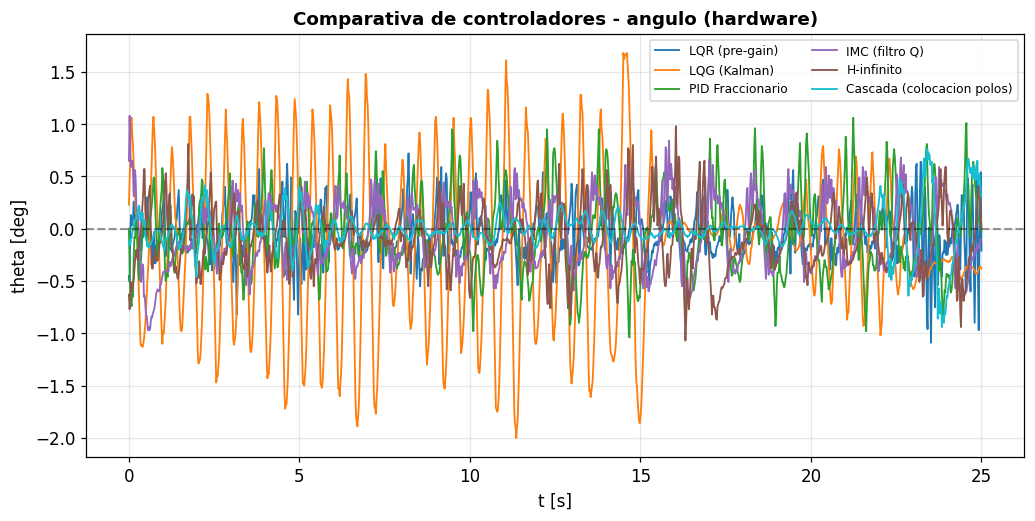
\includegraphics[width=0.48\textwidth]{comparativa.png}}
\caption{\'Angulo $\theta(t)$ de los seis controladores en hardware.}
\label{fig:comparativa}
\end{figure}

Todos los controladores mantienen el robot en pie con
$\theta_{RMS}<0.75^\circ$ y sin saturar el actuador. El \textbf{control en cascada}
corregido alcanza la mayor precisi\'on ($0.19^\circ$) con el menor esfuerzo
($|u|_{max}=32$, $u_{RMS}=4.8$), seguido por el \textbf{LQR} ($0.23^\circ$) y el
\textbf{$H_\infty$} ($0.30^\circ$). El \textbf{IMC} y el \textbf{FOPID} logran
$0.33$ y $0.36^\circ$ respectivamente, mientras que el \textbf{LQG} presenta el
mayor error ($0.73^\circ$), atribuible al retardo introducido por el observador
frente a estados que en esta planta ya son directamente medibles. La deriva de
posici\'on fue peque\~na en todos los casos ($\Delta x<0.2$ m) al mantenerse el
lazo de posici\'on desactivado durante la caracterizaci\'on angular.

\begin{figure*}[htbp]
\centering
\begin{minipage}{0.32\textwidth}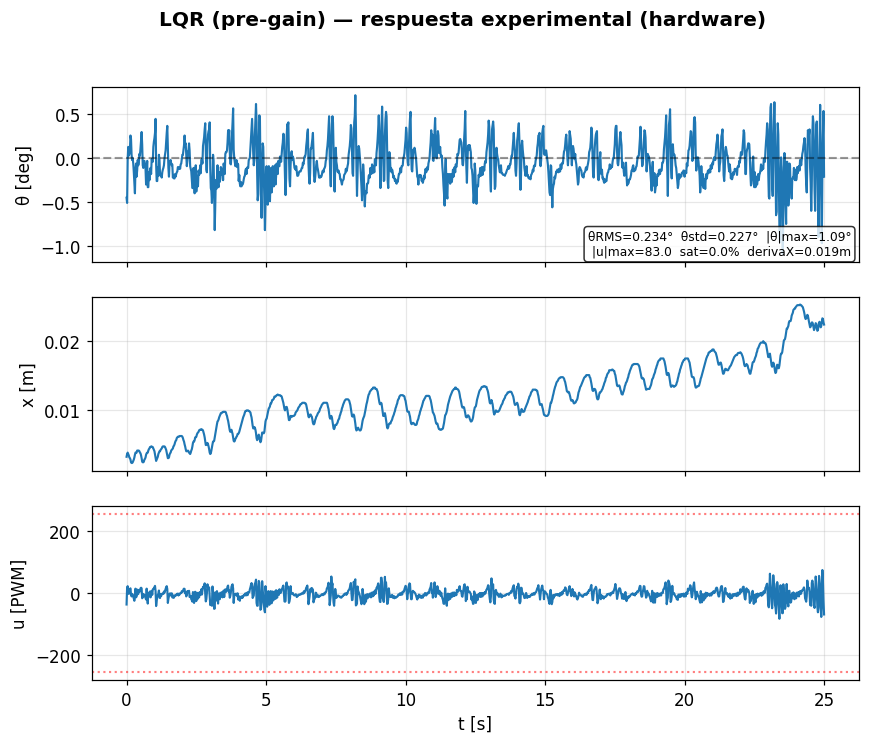
\includegraphics[width=\textwidth]{lqr.png}\\ \centering (a) LQR\end{minipage}\hfill
\begin{minipage}{0.32\textwidth}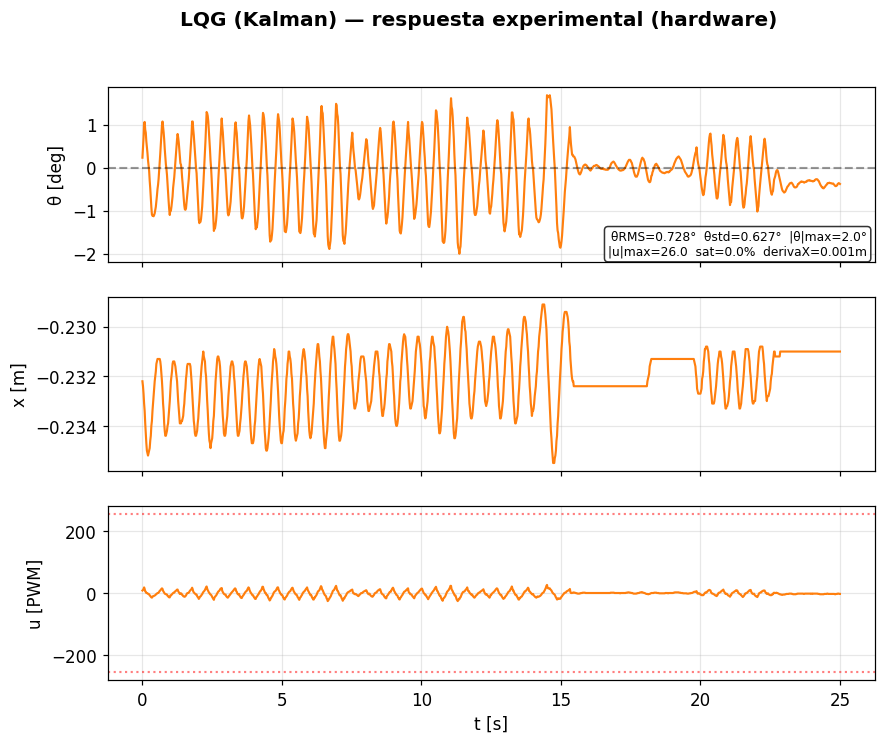
\includegraphics[width=\textwidth]{lqg.png}\\ \centering (b) LQG\end{minipage}\hfill
\begin{minipage}{0.32\textwidth}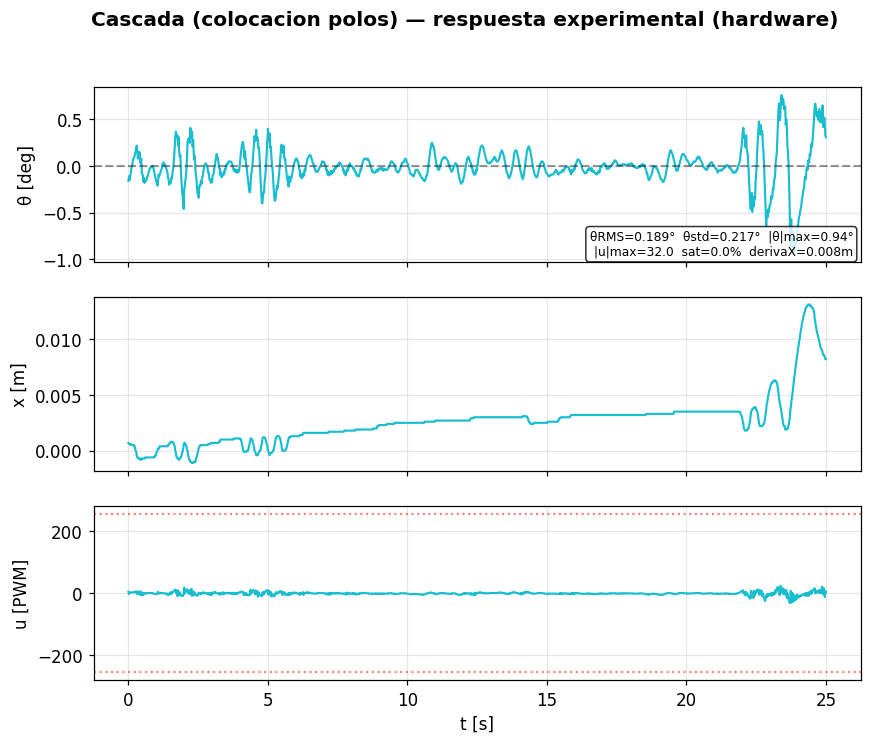
\includegraphics[width=\textwidth]{cascada.png}\\ \centering (c) Cascada\end{minipage}

\vspace{2mm}
\begin{minipage}{0.32\textwidth}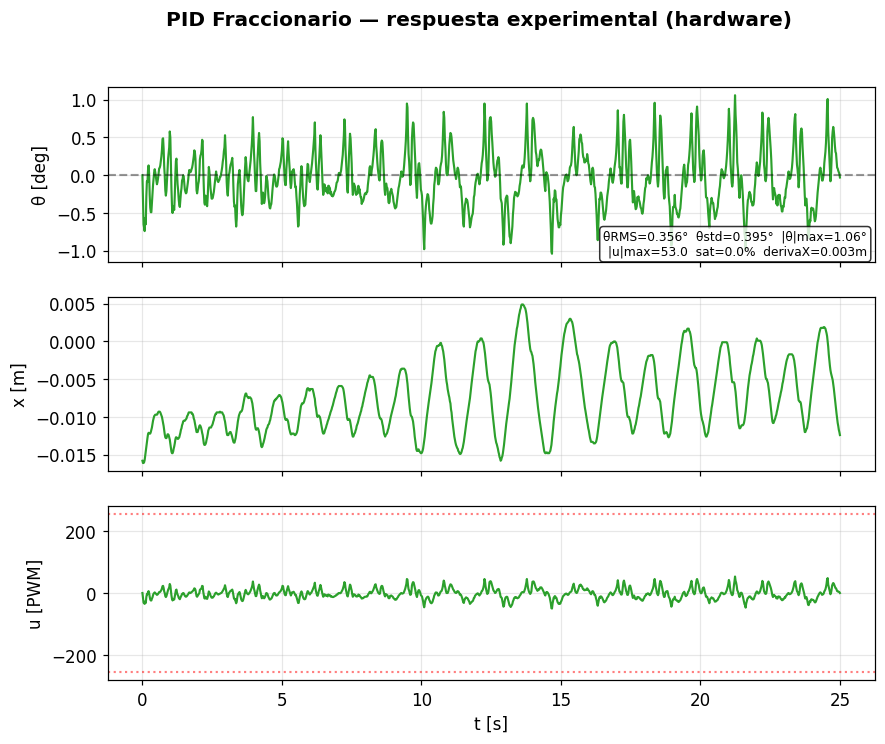
\includegraphics[width=\textwidth]{fopid.png}\\ \centering (d) FOPID\end{minipage}\hfill
\begin{minipage}{0.32\textwidth}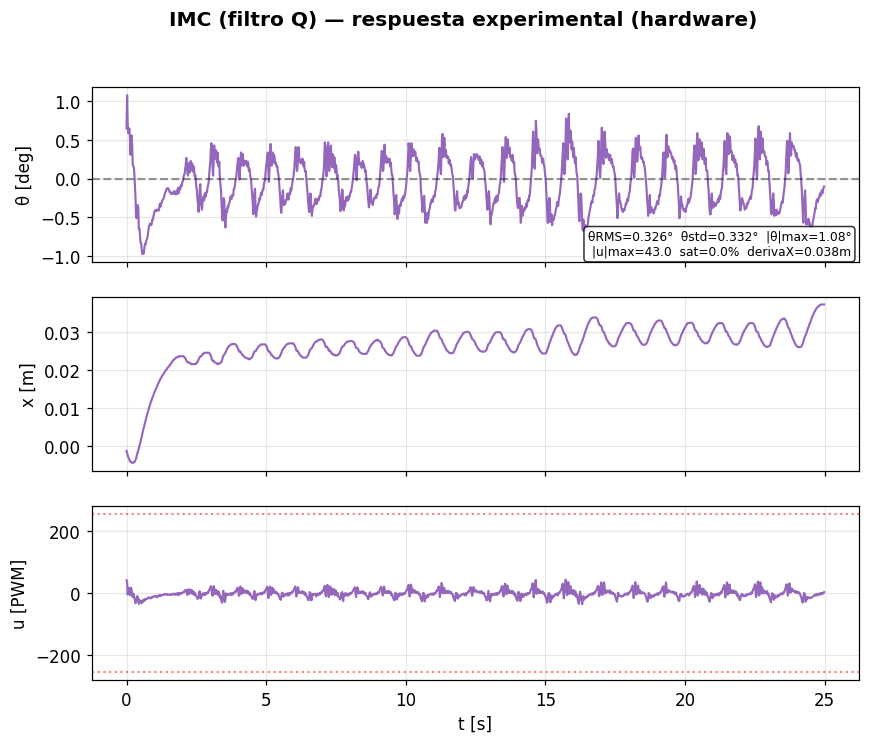
\includegraphics[width=\textwidth]{imc.png}\\ \centering (e) IMC\end{minipage}\hfill
\begin{minipage}{0.32\textwidth}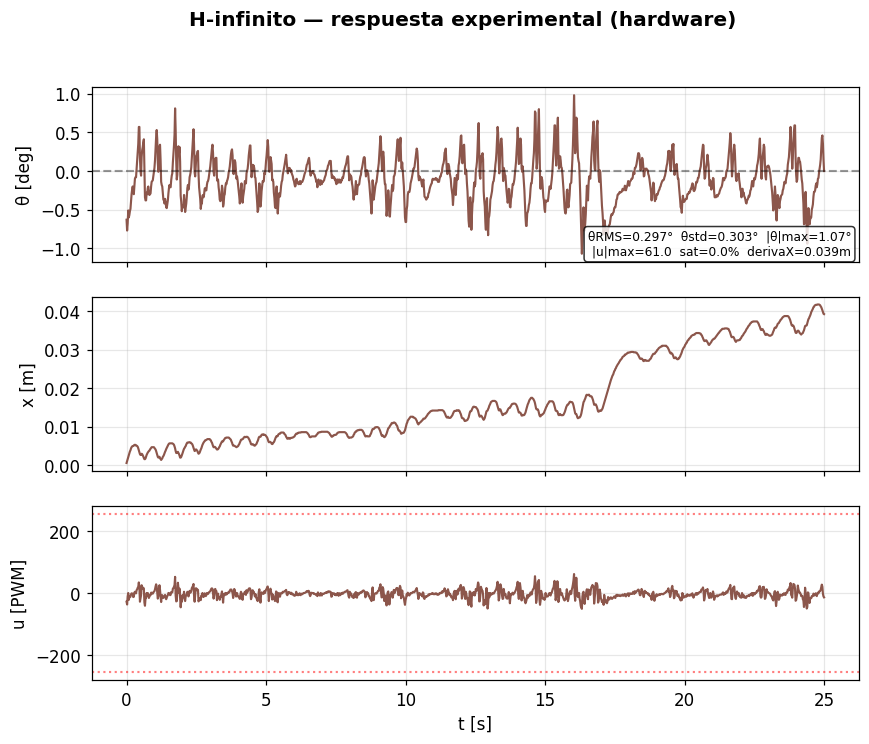
\includegraphics[width=\textwidth]{hinf.png}\\ \centering (f) $H_\infty$\end{minipage}
\caption{Respuesta experimental individual de cada controlador: \'angulo $\theta$, posici\'on $x$ y esfuerzo de control $u$.}
\label{fig:individuales}
\end{figure*}

\section{Discusi\'on}
\subsection{Compromiso desempe\~no--esfuerzo}
Existe una relaci\'on inversa entre precisi\'on y suavidad: la cascada y el LQR
logran bajo $\theta_{RMS}$ con esfuerzo moderado, mientras que el LQG usa el menor
$|u|_{max}$ pero a costa de mayor error. Esto refleja el ajuste de los pesos
($\mat{Q}$, $R$) y la din\'amica del observador.

\subsection{Correspondencia simulaci\'on--hardware}
La coincidencia es alta para LQR, LQG, IMC y cascada (mismo orden de magnitud). En
cambio, FOPID y $H_\infty$ \emph{no estabilizan el modelo lineal simplificado} con
las mismas ganancias, pero s\'i el robot real ($0.30$--$0.36^\circ$). La raz\'on
es que el modelo lineal no captura el amortiguamiento mec\'anico ni la din\'amica
del sensor, por lo que la planta f\'isica resulta m\'as tolerante. Este resultado
subraya que la validez de una simulaci\'on depende de la sensibilidad de cada
m\'etodo a las incertidumbres del modelo, y que la verificaci\'on experimental es
imprescindible.

\subsection{Lecci\'on de dise\~no: cancelaci\'on de polos}
El an\'alisis de la cascada evidenci\'o que \emph{cancelar} un polo inestable con
un cero del controlador conduce a inestabilidad interna, aunque la funci\'on de
transferencia lo oculte. La versi\'on por \emph{colocaci\'on} de polos, que
estabiliza genuinamente el modo inestable, result\'o adem\'as la de mejor
desempe\~no global.

\subsection{Limitaciones}
La caracterizaci\'on se centr\'o en la regulaci\'on angular con el lazo de
posici\'on desactivado; el seguimiento de trayectorias y el rechazo de
perturbaciones externas quedan como trabajo futuro, as\'i como una campa\~na
estad\'istica con m\'ultiples ensayos por controlador.

\section{Conclusiones}
Sobre una misma planta identificada y un mismo hardware se dise\~naron,
implementaron y compararon seis controladores para un veh\'iculo uniaxial tipo
p\'endulo invertido. Los seis estabilizan el robot con error sub-grado; el control
en cascada por colocaci\'on de polos ofreci\'o el mejor compromiso
desempe\~no/esfuerzo ($\theta_{RMS}=0.19^\circ$), seguido del LQR. La metodolog\'ia
uniforme de dise\~no y de extracci\'on de datos permiti\'o una comparaci\'on
objetiva y revel\'o tanto los l\'imites del modelo lineal para los controladores
m\'as sensibles como la importancia de estabilizar --y no cancelar-- los modos
inestables de la planta.

\begin{thebibliography}{00}
\bibitem{ogata} K. Ogata, \textit{Ingenier\'ia de Control Moderna}, 5\textsuperscript{a} ed. Madrid: Pearson, 2010.
\bibitem{astrom} K. J. \r{A}str\"om and R. M. Murray, \textit{Feedback Systems: An Introduction for Scientists and Engineers}. Princeton, NJ: Princeton Univ.\ Press, 2008.
\bibitem{skogestad} S. Skogestad and I. Postlethwaite, \textit{Multivariable Feedback Control: Analysis and Design}, 2\textsuperscript{nd} ed. Chichester, U.K.: Wiley, 2005.
\bibitem{anderson} B. D. O. Anderson and J. B. Moore, \textit{Optimal Control: Linear Quadratic Methods}. Englewood Cliffs, NJ: Prentice-Hall, 1990.
\bibitem{monje} C. A. Monje, Y. Chen, B. M. Vinagre, D. Xue, and V. Feliu, \textit{Fractional-order Systems and Controls: Fundamentals and Applications}. London, U.K.: Springer, 2010.
\bibitem{morari} M. Morari and E. Zafiriou, \textit{Robust Process Control}. Englewood Cliffs, NJ: Prentice-Hall, 1989.
\bibitem{gandarilla} I. Gandarilla \textit{et al.}, ``Trajectory tracking control of a self-balancing robot via adaptive neural networks,'' \textit{Eng.\ Sci.\ Technol., Int.\ J.}, vol.\ 35, 2022.
\end{thebibliography}

\end{document}
